\documentclass[11pt,letterpaper]{article}
\usepackage{fontspec}
\setmainfont{texgyrepagella}[Extension=.otf,UprightFont=*-regular,BoldFont=*-bold,ItalicFont=*-italic,BoldItalicFont=*-bolditalic]
\usepackage[bidi=default]{babel}
\babelprovide[import,main]{spanish}
\babelprovide[import]{hebrew}
\babelprovide[import]{ancientgreek}
\babelfont[hebrew]{rm}[Path=fonts/,BoldFont=NotoHebrewSerif-700.ttf,Scale=0.95]{NotoHebrewSerif-400.ttf}
\babelfont[ancientgreek]{rm}[Path=fonts/]{GFSPorson.otf}
\newcommand{\heb}[1]{\mbox{\foreignlanguage{hebrew}{#1}}}
\newcommand{\grc}[1]{\foreignlanguage{ancientgreek}{#1}}
\newcommand{\hebverso}[1]{\par\smallskip{\centering\begin{otherlanguage}{hebrew}\large #1\end{otherlanguage}\par}\smallskip}
\usepackage[margin=2.5cm,headheight=14pt]{geometry}
\usepackage{microtype,ragged2e,booktabs,graphicx,xcolor,csquotes,array}
\usepackage[hidelinks]{hyperref}\usepackage{xurl}\urlstyle{same}
\usepackage[most]{tcolorbox}
\usepackage{tikz}\usetikzlibrary{arrows.meta,positioning,calc,decorations.pathreplacing}
\usepackage{titlesec,fancyhdr,extramarks}
% Paleta "Israel": celeste y azul del tejelet (Nm 15:38) con oro del santuario
% (nombres conservados por compatibilidad: ladrillo = azul tejelet, cafe = azul real, cafeosc = azul noche,
%  piedra = celeste claro, sepia = azul pizarra)
\definecolor{cafe}{RGB}{26,82,150}\definecolor{cafeosc}{RGB}{11,33,74}\definecolor{tinta}{RGB}{20,32,56}
\definecolor{oro}{RGB}{206,162,52}\definecolor{ladrillo}{RGB}{20,68,140}
\definecolor{piedra}{RGB}{234,243,251}\definecolor{sepia}{RGB}{72,102,140}\definecolor{celeste}{RGB}{96,166,222}
\titleformat{\section}{\Large\bfseries\color{ladrillo}}{\thesection.}{0.6em}{}
\titleformat{\subsection}{\large\bfseries\color{cafe}}{\thesubsection}{0.6em}{}
\pagestyle{fancy}\fancyhf{}
\fancyhead[L]{\foreignlanguage{spanish}{\small\itshape\color{sepia}\firstleftmark}}\fancyhead[R]{\foreignlanguage{spanish}{\small\color{sepia}\thepage}}
\renewcommand{\sectionmark}[1]{\markboth{#1}{}}
\setlength{\parindent}{1.27cm}\linespread{1.15}\setlength{\emergencystretch}{3em}
\newtcolorbox{cita}[1][]{enhanced,colback=piedra,colframe=oro!90!ladrillo,boxrule=0pt,leftrule=2.5pt,arc=0pt,
  left=8pt,right=8pt,top=5pt,bottom=5pt,before skip=8pt,after skip=8pt,fontupper=\itshape,#1}
\newcommand{\fuente}[1]{\par\hfill{\upshape\bfseries\small\textcolor{ladrillo}{#1}}}
\newtcolorbox{nota}[1][]{enhanced,colback=oro!12,colframe=oro!80!ladrillo,boxrule=0.6pt,arc=2pt,
  fonttitle=\bfseries\small,coltitle=cafe,colbacktitle=oro!35,fontupper=\small,title={#1}}
\newcommand{\refapa}[1]{\par{\RaggedRight\hangindent=1.27cm\hangafter=1\noindent #1\par}\vspace{4pt}}
\newcommand{\destacar}[1]{\textbf{\textcolor{ladrillo}{#1}}}
\title{\color{ladrillo}\bfseries De los Jueces a David\\[4pt]\large\color{cafe}\mdseries Un pueblo que quiso ser como las naciones y un remanente que esperó al rey según el corazón de Dios}
\author{}\date{\color{sepia}Serie «Israel, el pueblo de Dios» · Estudio 3}
\begin{document}
\maketitle\thispagestyle{empty}

\begin{abstract}\noindent
Este tercer estudio recorre la historia de Israel desde la muerte de Josué hasta la muerte de Saúl y la unción de David, la etapa en que el pueblo llamado a ser «reino de sacerdotes y nación santa» (Éx 19:6) pidió ser «como todas las naciones» (1~S 8:5, 20). Jueces narra una espiral descendente en la que la vocación sacerdotal de Israel se quiebra desde dentro (un levita a sueldo, un santuario idolátrico en Dan, los hijos de Elí), hasta que en Guibeá el pueblo repite el pecado de Sodoma; el estribillo «no había rey en Israel; cada uno hacía lo que bien le parecía» (Jue 17:6; 21:25) da nombre a esa ruina. Sin embargo, en medio del desastre Dios preserva un remanente (Débora, Rut la moabita, Ana, Samuel, Jonatán, David) y anuncia por primera vez un rey «ungido» (\emph{mashíaj}, 1~S 2:10), una esperanza que Isaías, Jeremías, Oseas y Miqueas proyectan hacia el futuro y que Pablo retoma en Ro 1:3 y 11:1--5. El análisis se apoya en el texto hebreo y sus variantes de Qumrán, en la arqueología del Hierro~I con sus debates (aldeas de la sierra, Silo, filisteos de Ecrón y Gat, Bet-semes, Khirbet Qeiyafa) y en la tradición judía (Seder Olam, Talmud, Midrash, Targum, Josefo, haftarot y Shavuot).
\par\smallskip\noindent\textbf{Palabras clave:} Jueces, Rut, Samuel, Saúl, David, ungido, remanente, Isaías, Jeremías, Romanos 11.
\end{abstract}

\section{Introducción}

¿Qué ocurre cuando el pueblo de Dios se cansa de ser distinto? Jueces, Rut y 1~Samuel responden con una historia de casi dos siglos en la que Israel, ya instalado en la tierra, sirve a los baales de sus vecinos y acaba pidiendo un rey «como todas las naciones» (1~S 8:5). Mucho después, cuando Pablo se pregunte si Dios ha desechado a su pueblo, contestará con una frase que procede de esta misma etapa: «No ha desechado Dios a su pueblo» (Ro 11:2; cf. 1~S 12:22).

La vocación de Israel no se pierde aquí por la presión de cananeos y filisteos. Se pierde desde dentro, porque levitas, sacerdotes y tribus hacen «lo recto ante sus propios ojos» en lugar de lo recto ante los ojos de YHWH (Dt 12:8, 25). Con todo, Dios no suelta su promesa: levanta libertadores, guarda un remanente, incorpora a una moabita al linaje de Judá y, por boca de una mujer que había sido estéril, anuncia un rey ungido. Los profetas proyectarán esa esperanza hacia la restauración final, y Pablo la verá cumplida en el Mesías «del linaje de David según la carne» (Ro 1:3).

\begin{center}\small
\renewcommand{\arraystretch}{1.3}
\begin{tabular}{>{\RaggedRight\arraybackslash}p{3.1cm}>{\RaggedRight\arraybackslash}p{5.6cm}>{\RaggedRight\arraybackslash}p{5.2cm}}
\toprule
\textbf{Eje de la serie} & \textbf{Pregunta en esta etapa} & \textbf{Textos centrales}\\
\midrule
Nación santa y reino de sacerdotes & ¿Cómo se quiebra la vocación sacerdotal de Israel y quiénes la preservan? & Jue 2:11--19; 17--21; Rt 1:16--17; 1~S 2:12--36; 8:5--7; 12:23\\
Promesa de restauración & ¿Qué esperanza nace en medio de la ruina? & Jue 2:16--18; Rt 4:14--17; 1~S 2:10, 35; 12:22; 16:1--13\\
Proyección profética y paulina & ¿Cómo releen Isaías, Jeremías, Oseas y Pablo esta etapa? & Is 1:26; 9:4 [9:3]; 11:1; Jer 23:5--6; Os 3:4--5; Hch 13:16--23; Ro 11:1--5\\
\bottomrule
\end{tabular}\end{center}

\begin{nota}[Sobre traducción, numeración y fechas]
Las citas bíblicas son traducción propia desde el texto hebreo (BHS) y griego (NA28); la Septuaginta se cita según Rahlfs-Hanhart, y los fragmentos de Samuel de Qumrán (4QSam\textsuperscript{a}) según Cross et~al. (2005). Cuando la numeración hebrea difiere de la española, se da la española y la hebrea entre corchetes, por ejemplo Is 9:4 [9:3] o Mi 5:2 [5:1]. En esta etapa «Israel» designa a todo el pueblo de las doce tribus; cuando un texto distingue ya entre «Israel» y «Judá» (1~S 11:8; 18:16; 2~S 2:4, 9--10) se indica. Fechas en a.\,e.\,c. y e.\,c.
\end{nota}

\section{Marco cronológico}

El período va desde la muerte de Josué (Jue 2:8) hasta la muerte de Saúl en Gilboa (1~S 31) y la unción de David como rey de Judá en Hebrón (2~S 2:4). La cronología convencional lo sitúa, de modo aproximado, entre c.~1200 y c.~1010 a.\,e.\,c., en la Edad del Hierro~I; Saúl habría reinado hacia c.~1025--1010 y David desde c.~1010 a.\,e.\,c. (2~S 5:4--5).

Los datos bíblicos, por su parte, no encajan con facilidad. 1~R 6:1 cuenta 480 años desde el Éxodo hasta el cuarto año de Salomón, mientras que la suma sucesiva de opresiones, judicaturas y reposos de Jueces da unos 390 años (cálculo propio, con los veinte años de Sansón dentro de los cuarenta de opresión filistea, Jue 13:1; 15:20), y, si se añaden el desierto, Josué, Elí (1~S 4:18), Samuel, Saúl y David, la cifra se excede. De ahí que muchos intérpretes entiendan que varios jueces fueron regionales y que sus períodos se superponen: Jue 10:7 menciona a la vez a los amonitas al este y a los filisteos al oeste. La cronología rabínica de Seder Olam Rabbah ajusta las cifras de Jueces a los 480 años de 1~R 6:1 (Guggenheimer, 1998).

\begin{nota}[Precisión textual: Hch 13:20 y 1~S 13:1]
En Antioquía de Pisidia, Pablo dice según el texto crítico (NA28) que Dios dio a Israel la tierra «por unos cuatrocientos cincuenta años; y después de esto les dio jueces» (\grc{ὡς ἔτεσιν τετρακοσίοις καὶ πεντήκοντα. καὶ μετὰ ταῦτα ἔδωκεν κριτάς}): los 450 años cubren Egipto, el desierto y la conquista. El texto bizantino, que sigue la Reina-Valera, aplica la cifra al período de los jueces. Este estudio sigue el texto crítico.\par\smallskip
En 1~S 13:1 el TM dice literalmente que Saúl «tenía un año» al comenzar a reinar y que «reinó dos años»: casi con seguridad se perdieron cifras en la copia, y la Septuaginta antigua omite el versículo. Pablo le atribuye cuarenta años (Hch 13:21); Josefo da cifras distintas en lugares distintos. Este estudio no fija la duración del reinado de Saúl.
\end{nota}

\begin{center}
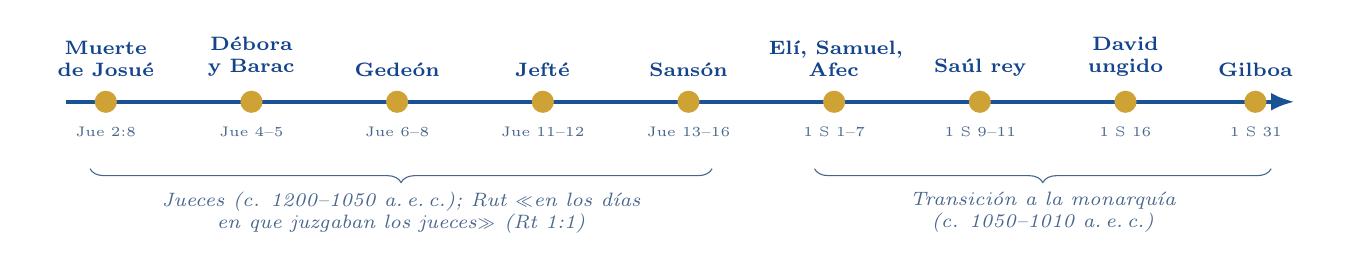
\begin{tikzpicture}[x=1cm,y=1cm]
\draw[line width=1.6pt,cafe,-{Latex[length=3mm]}] (0,0) -- (15.6,0);
\foreach \x/\t/\b in {0.5/{Muerte de Josué}/{Jue 2:8},
                      2.35/{Débora y Barac}/{Jue 4--5},
                      4.2/{Gedeón}/{Jue 6--8},
                      6.05/{Jefté}/{Jue 11--12},
                      7.9/{Sansón}/{Jue 13--16},
                      9.75/{Elí, Samuel, Afec}/{1~S 1--7},
                      11.6/{Saúl rey}/{1~S 9--11},
                      13.45/{David ungido}/{1~S 16},
                      15.1/{Gilboa}/{1~S 31}}{
  \fill[oro] (\x,0) circle (4pt);
  \node[above,font=\scriptsize\bfseries,text=ladrillo,text width=1.75cm,align=center] at (\x,0.2) {\t};
  \node[below,font=\tiny,text=sepia,text width=1.7cm,align=center] at (\x,-0.2) {\b};}
\draw[decorate,decoration={brace,amplitude=5pt,mirror},sepia] (0.3,-0.85) -- (8.2,-0.85) node[midway,below=5pt,font=\scriptsize\itshape,align=center]{Jueces (c. 1200--1050 a.\,e.\,c.); Rut «en los días\\ en que juzgaban los jueces» (Rt 1:1)};
\draw[decorate,decoration={brace,amplitude=5pt,mirror},sepia] (9.5,-0.85) -- (15.3,-0.85) node[midway,below=5pt,font=\scriptsize\itshape,align=center]{Transición a la monarquía\\(c. 1050--1010 a.\,e.\,c.)};
\end{tikzpicture}\\[2pt]
{\footnotesize\color{sepia}\textit{Nota.} Elaboración propia. Secuencia narrativa; las fechas absolutas son aproximadas y están en debate.}
\end{center}

\section{Contexto histórico y arqueológico}

\subsection{Las aldeas de la sierra central}
Las prospecciones de la sierra central (Efraín, Manasés, Benjamín y el norte de Judá) muestran un cambio notable entre el Bronce Tardío y el Hierro~I: de unas pocas decenas de sitios se pasa a más de doscientas cincuenta pequeñas aldeas sin murallas (Finkelstein, 1988). Comparten la casa de cuatro espacios con pilares, cisternas revocadas, terrazas agrícolas y jarras de borde con collar. Stager (1985) mostró que esa casa se ajusta bien a la familia extendida que Jueces llama \emph{bet av}, «casa del padre» (Jue 6:15). El cuadro coincide con el Israel que describe el libro: aldeas sin capital, sin rey y sin ejército permanente, cuyas tribus solo se congregan cuando las amenaza un enemigo. La Estela de Merneptah (c.~1208 a.\,e.\,c., Estudio~1) confirma que Israel ya existía como pueblo en Canaán al comienzo del período.

\begin{center}\begin{minipage}{\linewidth}\centering
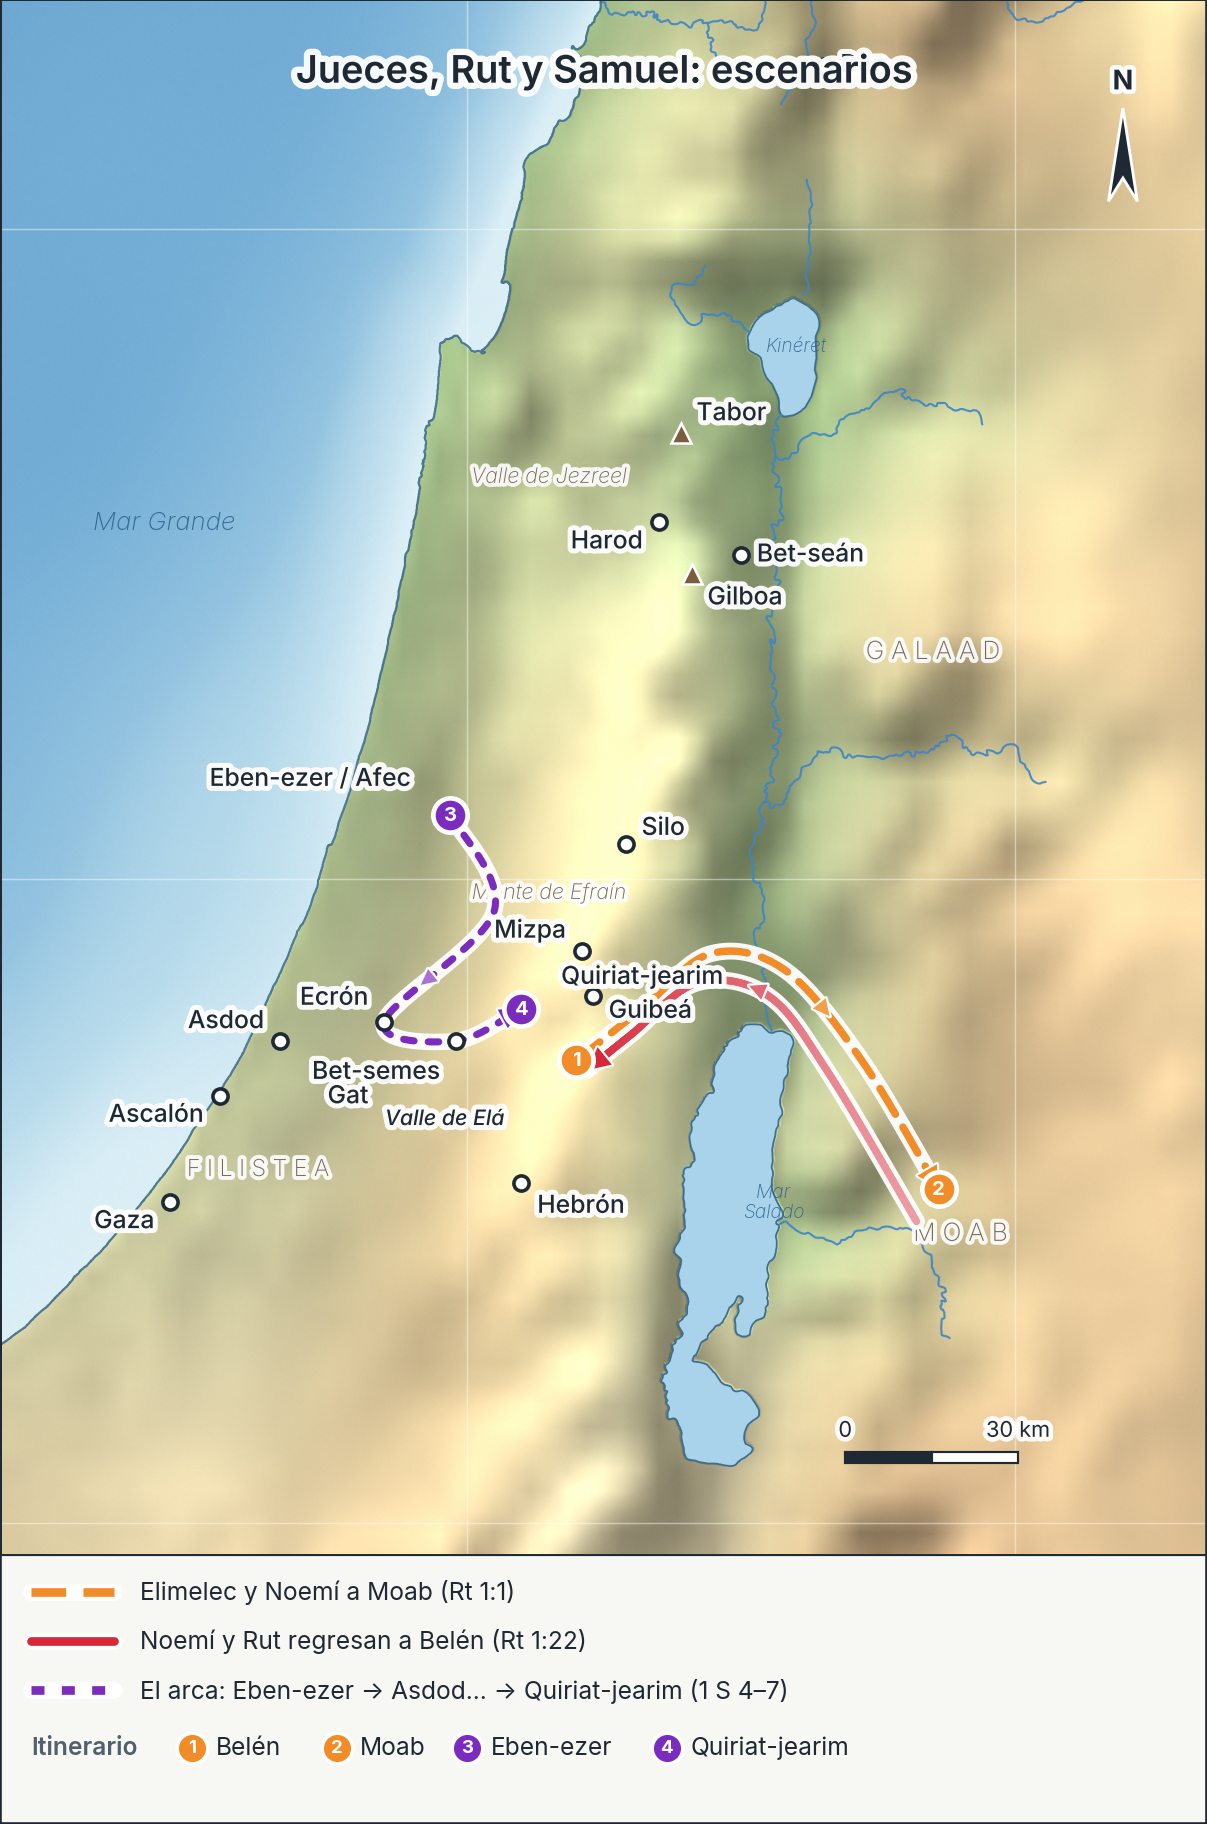
\includegraphics[width=0.62\linewidth]{mapa_jueces.png}\\[2pt]
{\footnotesize\color{sepia}\textit{Nota.} Elaboración propia: costas, lagos y ríos GSHHS/WDB y relieve sombreado (Basemap); ubicaciones antiguas aproximadas. }
\end{minipage}\end{center}


\begin{nota}[Debate: la ausencia de cerdo y la identidad israelita]
En las aldeas de la sierra casi no aparecen huesos de cerdo, mientras que en las ciudades filisteas son frecuentes. Faust (2006) lo interpreta como un marcador de identidad israelita, coherente con Lv 11:7. Hesse y Wapnish (1997) advierten que la cría de cerdos depende también del clima y la economía, y que otros pueblos tampoco los criaban, de modo que la ausencia de cerdo no basta por sí sola para identificar un sitio como israelita. Lo mismo vale para la casa de cuatro espacios o la jarra con collar, que no son exclusivas. La cuestión sigue abierta.
\end{nota}

\subsection{Los filisteos}
En la segunda mitad del período el gran adversario son los filisteos (Jue 13--16; 1~S 4--31), llegados a la costa sur de Canaán con los «Pueblos del Mar»: los relieves de Medinet Habu muestran a Ramsés~III (c.~1177 a.\,e.\,c.) combatiendo, entre otros, a los \emph{Peleset}, el hebreo \heb{פְּלִשְׁתִּים} (\emph{pelishtím}). En Asdod, Ascalón, Ecrón y Gat aparece una cultura material de origen egeo: cerámica monocroma y luego bícroma, hogares de tipo egeo, consumo de cerdo (Dothan, 1982). Un estudio de ADN antiguo de Ascalón detectó en individuos del Hierro~I un componente de origen europeo meridional que se diluye en pocas generaciones (Feldman et~al., 2019). La Biblia conoce su organización: cinco ciudades gobernadas por \heb{סְרָנִים} (\emph{seraním}, Jue 3:3; 1~S 6:16--18), palabra que muchos relacionan con el griego \grc{τύραννος} (etimología en debate). Dos hallazgos rozan de cerca el relato bíblico:

\begin{itemize}
\item \textbf{La inscripción real de Ecrón} (Tel Miqne, 1996): dedicatoria de un templo por «Akish, hijo de Padi, rey de Ecrón» (Gitin et~al., 1997). Confirma la identificación del sitio y muestra que \emph{Akish} era un nombre real filisteo, el de Aquis, rey de Gat, en 1~S 21:10 [21:11] y 27:2. Es del siglo \textsc{vii} a.\,e.\,c. y no menciona al Aquis bíblico.
\item \textbf{El ostracón de Gat} (Tell es-Safi, 2005): un fragmento del Hierro~I tardío o IIA temprano con dos nombres, \emph{’LWT} y \emph{WLT}, de origen probablemente no semítico y etimológicamente cercanos a «Goliat» según sus editores (Maeir et~al., 2008). No menciona a Goliat, pero muestra que en Gat circulaban nombres de ese tipo; la relación lingüística, con todo, es una interpretación debatida.
\end{itemize}

Según 1~S 13:19--22, los israelitas bajaban a los filisteos a afilar sus herramientas y pagaban un \heb{פִּים} (\emph{pim}), palabra que los traductores antiguos no entendían; su sentido se aclaró cuando aparecieron pesas de piedra inscritas \emph{pym}, de unos dos tercios de siclo. La idea de un «monopolio filisteo del hierro», en cambio, es discutida.

\subsection{Silo, Eben-ezer, Bet-semes y Khirbet Qeiyafa}
\textbf{Silo} (Khirbet Seilun), excavada por Finkelstein entre 1981 y 1984, tenía en el Hierro~I edificios con pilares y depósitos, y fue destruida por un incendio hacia mediados del siglo \textsc{xi} a.\,e.\,c. (Finkelstein et~al., 1993). Muchos asocian esa destrucción con la derrota de Afec (1~S 4), aunque Samuel no narra la caída de Silo; son Jer 7:12--14 y Sal 78:60 los que la recuerdan. Las excavaciones recientes en el sitio todavía están en proceso de publicación y discusión. \textbf{Eben-ezer} se ha identificado, con dudas, con \emph{Izbet Sartah}, aldea frente a Afec donde apareció un abecedario protocananeo. \textbf{Bet-semes}, adonde vuelve el arca (1~S 6), era una población fronteriza con la llanura filistea, y sus excavadores ven en la escasez de cerdo del Hierro~I una frontera cultural consciente frente a Ecrón (Bunimovitz y Lederman, 2009), con el debate ya señalado.

\textbf{Khirbet Qeiyafa}, sobre el valle de Ela donde 1~S 17 sitúa el combate con Goliat, es una fortaleza de unas 2,3 hectáreas con muralla de casamatas y dos puertas, fechada por radiocarbono hacia c.~1020--980 a.\,e.\,c. Sus excavadores la consideran una ciudad de Judá del tiempo de David y proponen identificarla con Saaraim, «las dos puertas» (1~S 17:52; Garfinkel et~al., 2016). Finkelstein y Fantalkin (2012) aceptan la fecha, pero atribuyen el sitio a una entidad del norte, posiblemente la de Saúl, y no faltan quienes lo consideran cananeo o filisteo.

\begin{nota}[Debate: la «cronología baja»]
Finkelstein propuso bajar unos ochenta o cien años las fechas del Hierro~I y IIA, lo que reduciría el reino de David a un pequeño cacicazgo. Mazar (1990) y otros mantienen una cronología convencional o modificada. Khirbet Qeiyafa y la Estela de Tel Dan («casa de David», Estudio~4) alimentan el debate en ambos sentidos.
\end{nota}

\section{Desarrollo bíblico}

\subsection{El ciclo de los jueces y su espiral descendente (Jue 2:11--19)}
Antes de contar ninguna historia, el prólogo teológico de Jueces ofrece la clave de lectura de todo el libro:

\hebverso{וַיַּעֲשׂוּ בְנֵי־יִשְׂרָאֵל אֶת־הָרַע בְּעֵינֵי יְהוָה וַיַּעַבְדוּ אֶת־הַבְּעָלִים\\
וַיָּקֶם יְהוָה שֹׁפְטִים וַיּוֹשִׁיעוּם מִיַּד שֹׁסֵיהֶם}
\begin{cita}Y los hijos de Israel hicieron lo malo ante los ojos de YHWH y sirvieron a los baales [\ldots]. Y YHWH levantó jueces que los libraron de mano de los que los saqueaban [\ldots], porque YHWH se compadecía de su gemido. Pero cuando moría el juez, volvían a corromperse más que sus padres.\fuente{(Jue 2:11, 16, 18--19)}\end{cita}

El ciclo consta de cinco momentos: apostasía, opresión, clamor (\heb{וַיִּזְעֲקוּ}, \emph{va-yiz'aqú}, Jue 3:9; 6:6), libertador y reposo. El v.~19, sin embargo, añade que cada generación se corrompe \emph{más} que la anterior, y el relato lo confirma. La fórmula «y reposó la tierra» aparece tras Otoniel, Aod, Débora y Gedeón (3:11, 30; 5:31; 8:28) y después ya no vuelve; la unidad de las tribus se deshace hasta desembocar en guerra civil (8:1; 12:1--6; 15:11--13; Jue 20), y la talla moral de los propios jueces va menguando. Conviene precisar que el \heb{שֹׁפֵט} (\emph{shofet}) no es un magistrado de tribunal, sino un líder carismático que libra y gobierna; el texto insiste en que es YHWH quien lo «levanta», porque el verdadero juez es Él (Jue 11:27).

\begin{center}
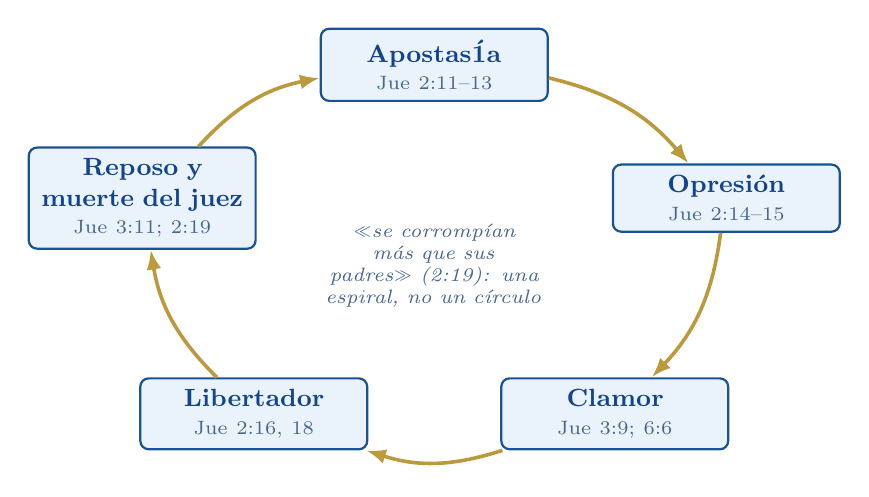
\begin{tikzpicture}[every node/.style={font=\small}]
\foreach \a/\t/\r [count=\i] in {90/{Apostasía}/{2:11--13},18/{Opresión}/{2:14--15},-54/{Clamor}/{3:9; 6:6},-126/{Libertador}/{2:16, 18},162/{Reposo y muerte del juez}/{3:11; 2:19}}{
  \node[draw=cafe,line width=0.8pt,fill=piedra,rounded corners=3pt,text width=2.6cm,align=center,inner sep=4pt] (c\i) at ({3.9*cos(\a)},{2.45*sin(\a)}) {\textbf{\textcolor{ladrillo}{\t}}\\[-1pt]{\scriptsize\color{sepia}Jue \r}};}
\foreach \a/\b in {1/2,2/3,3/4,4/5,5/1}{\draw[-{Latex[length=2.5mm]},oro!90!ladrillo,line width=1.3pt] (c\a) to[bend left=18] (c\b);}
\node[text width=2.8cm,align=center,font=\scriptsize\itshape,text=sepia] at (0,-0.1) {«se corrompían más que sus padres» (2:19): una espiral, no un círculo};
\end{tikzpicture}\\[2pt]
{\footnotesize\color{sepia}\textit{Nota.} Elaboración propia a partir de Jue 2:11--19.}
\end{center}

\begin{center}\small
\renewcommand{\arraystretch}{1.2}
\begin{tabular}{>{\RaggedRight\arraybackslash}p{2.0cm}>{\RaggedRight\arraybackslash}p{2.1cm}>{\RaggedRight\arraybackslash}p{2.5cm}>{\RaggedRight\arraybackslash}p{1.6cm}>{\RaggedRight\arraybackslash}p{5.6cm}}
\toprule
\textbf{Juez} & \textbf{Tribu} & \textbf{Opresor} & \textbf{Texto} & \textbf{Rasgo}\\
\midrule
Otoniel & Judá & Cusán-risataim & 3:7--11 & Modelo inicial: el Espíritu viene sobre él; reposo de 40 años\\
Aod & Benjamín & Eglón de Moab & 3:12--30 & Libertador zurdo; la tierra reposa 80 años\\
Débora y Barac & Efraín\,/ Neftalí & Jabín y Sísara & 4--5 & Profetisa y jueza; Jael completa la victoria\\
Gedeón & Manasés & Madián & 6--8 & Rechaza la corona (8:23), pero su efod se vuelve tropiezo\\
Jefté & Galaad & Amón & 10:6--12:7 & Voto temerario; guerra contra Efraín («shibólet»)\\
Sansón & Dan & Filisteos & 13--16 & Nazareo desde el vientre; vive «según sus ojos»\\
\bottomrule
\end{tabular}\\[2pt]
{\footnotesize\color{sepia}\textit{Nota.} Elaboración propia. Se omiten los «jueces menores» (Samgar, Tola, Jair, Ibzán, Elón, Abdón).}
\end{center}

\subsection{Débora, Gedeón y Jefté}
\textbf{Débora}, «profetisa» que «juzgaba a Israel» (Jue 4:4), convoca a Barac contra Sísara, y la victoria la consuma otra mujer, Jael. Lo que Jue 4 narra, Jue 5 lo canta. Muchos especialistas tienen el cántico de Débora, junto con Éx 15, por uno de los poemas más antiguos de la Biblia, a causa de su hebreo arcaico y de su imagen de unas tribus sin monarquía (Cross y Freedman, 1997); otros lo datan más tarde. El poema funciona como un balance de responsabilidades: alaba a Efraín, Benjamín, Maquir, Zabulón, Isacar y Neftalí, reprocha a Rubén, Galaad, Dan y Aser (5:14--18), maldice a Meroz «porque no vinieron en ayuda de YHWH» (5:23) y guarda silencio sobre Judá y Simeón. Para el poeta, Israel existe como pueblo cuando acude unido al llamado de Dios: «así perezcan todos tus enemigos, oh YHWH; pero los que le aman sean como el sol cuando sale en su fuerza» (5:31).

\textbf{Gedeón}, de Manasés, vence a Madián con trescientos hombres «para que Israel no se alabe contra mí» (7:2). Al ofrecérsele una dinastía, la rechaza con la fórmula que mejor expresa el ideal teocrático del período:

\hebverso{לֹא־אֶמְשֹׁל אֲנִי בָּכֶם וְלֹא־יִמְשֹׁל בְּנִי בָּכֶם יְהוָה יִמְשֹׁל בָּכֶם}
\begin{cita}No reinaré yo sobre vosotros, ni mi hijo reinará sobre vosotros; YHWH reinará sobre vosotros.\fuente{(Jue 8:23)}\end{cita}

Acto seguido, sin embargo, fabrica con el oro del botín un efod que «todo Israel prostituyó tras él» (8:27), y su hijo Abimelec («mi padre es rey») se hace rey en Siquem matando a setenta hermanos (Jue 9). La fábula de Jotam (9:7--15), donde solo la zarza acepta reinar, es la primera crítica bíblica a una monarquía nacida de la ambición. La victoria sobre Madián quedará en la memoria profética como figura de la liberación futura (Is 9:4 [9:3]; 10:26).

\textbf{Jefté}, hijo de una prostituta y expulsado por sus hermanos, conoce bien la historia del Éxodo (Jue 11:12--28); su voto, en cambio, delata hasta qué punto el período se ha contaminado. Promete ofrecer en holocausto lo primero que salga de su casa, y sale su hija única (11:30--40). La lectura más directa, y la de Josefo, que condena el acto (\emph{Antigüedades} 5.7.10), es que la sacrificó; algunos comentaristas judíos medievales, como David Kimji, propusieron que fue consagrada a la virginidad (11:39). Sea cual sea la lectura, el juez trata a YHWH con la lógica de los dioses vecinos (Lv 18:21; Dt 12:31). Poco después, los galaaditas degüellan a los efraimitas que no saben pronunciar \heb{שִׁבֹּלֶת} (\emph{shibólet}) y dicen \heb{סִבֹּלֶת} (\emph{sibólet}) (12:5--6): Israel ya ha empezado a matar a Israel.

\subsection{Sansón: el nazareo que vivió según sus ojos}
Como Isaac, Sansón nace de una mujer estéril tras un anuncio divino (Jue 13:2--3). Debía ser «nazareo de Dios desde el vientre» (\heb{נְזִיר אֱלֹהִים}, \emph{nezir Elohim}, 13:5), apartado según Nm 6, y «comenzará a salvar a Israel de mano de los filisteos»: una salvación que completarán Samuel y David (1~S 7:13; 2~S 8:1). Uno tras otro, Sansón quebranta los signos de su consagración: toca el cadáver del león (14:8--9), celebra un banquete de bebida (\heb{מִשְׁתֶּה}, \emph{mishté}, 14:10) y revela el secreto de su cabello (16:17). Lo que dice de la mujer filistea podría servirle de divisa: «tómamela, porque ella es recta a mis ojos» (\heb{כִּי־הִיא יָשְׁרָה בְעֵינָי}, 14:3), anticipo del estribillo final del libro. Acaba ciego en Gaza y muere derribando el templo de Dagón (16:21--30), y aun así Heb 11:32 lo cuenta entre los que actuaron «por la fe». En su figura se reconoce el Israel de la época, consagrado desde su origen, entregado a vivir como las naciones y, pese a todo, nunca despojado de su llamado.

\subsection{La vocación sacerdotal quebrada: Micaía y Dan (Jue 17--18)}
Los cinco capítulos finales de Jueces abandonan el ciclo y forman dos apéndices sobre la ruina interna del pueblo. El efraimita Micaía hace un ídolo con plata robada a su madre, monta un santuario con efod y terafines y contrata como sacerdote a un levita de Belén por diez siclos al año (17:1--13). Su conclusión lo dice todo: «Ahora sé que YHWH me prosperará, porque tengo un levita por sacerdote» (17:13); la religión se ha convertido en un recurso para asegurarse la bendición. Más tarde, la tribu de Dan emigra al norte, roba el ídolo y al levita, extermina a la pacífica Lais y funda un santuario que dura «hasta el día del cautiverio de la tierra» (18:30), dato que tiende un hilo entre esta etapa y el destierro asirio del reino del norte (Estudio~5), pues en el mismo Dan pondrá Jeroboam uno de sus becerros (1~R 12:29).

\begin{nota}[Precisión textual: el nieto de Moisés (Jue 18:30)]
El sacerdote de Dan es «Jonatán, hijo de Gersón, hijo de \emph{Manasés}». En el TM la \emph{nun} de \heb{מנשה} está escrita suspendida sobre la línea; sin ella se lee \heb{משה}, «Moisés», cuyo hijo era Gersón (Éx 2:22). El Talmud explica que se añadió para no avergonzar a Moisés con la idolatría de su nieto (Bava Batra 109b), y varios manuscritos de la Septuaginta y la Vulgata leen «Moisés». De ser así, el primer sacerdote idólatra de Israel fue nieto del mediador del Sinaí.
\end{nota}

\subsection{Guibeá y la guerra contra Benjamín (Jue 19--21)}
Un levita de Efraín vuelve de Belén con su concubina; no quiere pernoctar en Jebús «porque es ciudad de extranjeros» (19:12) y prefiere Guibeá de Benjamín. Allí los hombres de la ciudad rodean la casa y repiten casi palabra por palabra a los de Sodoma (19:22; cf. Gn 19:4--5). La concubina muere tras una noche de abuso, y el levita envía sus pedazos a las tribus. La inversión es deliberada y el narrador espera que el lector la advierta: Israel, que debía ser luz para Canaán, se ha convertido en Sodoma. La guerra que sigue deja a Benjamín al borde del exterminio, y el pueblo llora: «¿Por qué, oh YHWH, Dios de Israel, ha sucedido esto, que falte hoy de Israel una tribu?» (21:3). Siglos más tarde, Oseas evocará el episodio como el pecado que marca la medida de todos los demás: «desde los días de Guibeá has pecado, oh Israel» (\heb{מִימֵי הַגִּבְעָה חָטָאתָ יִשְׂרָאֵל}, Os 10:9; cf. 9:9). El libro se cierra con el estribillo que lo ha venido acompañando:

\hebverso{בַּיָּמִים הָהֵם אֵין מֶלֶךְ בְּיִשְׂרָאֵל אִישׁ הַיָּשָׁר בְּעֵינָיו יַעֲשֶׂה}
\begin{cita}En aquellos días no había rey en Israel; cada uno hacía lo que era recto ante sus propios ojos.\fuente{(Jue 21:25; cf. 17:6; 18:1; 19:1)}\end{cita}

La frase recoge la advertencia de Dt 12:8: «no haréis [\ldots] \emph{cada uno lo que es recto ante sus ojos}» (\heb{אִישׁ כָּל־הַיָּשָׁר בְּעֵינָיו}), en contraste con «lo recto ante los ojos de YHWH» (Dt 12:25, 28). Es un estribillo de doble filo. Prepara el terreno para la monarquía, pero deja intacto el ideal de Gedeón (Jue 8:23), porque lo que falta en Israel no es tanto un monarca como alguien que busque lo recto a los ojos de Dios.

\begin{nota}[Lectura literaria: Belén, Guibeá y Judá]
Varios intérpretes observan que los apéndices de Jueces preparan la historia de David (Block, 1999): los dos levitas están ligados a Belén, la ciudad de David; la villanía ocurre en Guibeá, la ciudad de Saúl (1~S 10:26); y el libro se abre y se cierra con la pregunta «¿quién subirá primero?» y la respuesta «Judá» (Jue 1:1--2; 20:18). Se trata de una lectura de la composición, no de un dato explícito del texto.
\end{nota}

\subsection{Rut: la moabita que eligió al Dios de Israel}
Rut ocurre «en los días en que juzgaban los jueces» (\heb{וַיְהִי בִּימֵי שְׁפֹט הַשֹּׁפְטִים}, Rt 1:1) y comparte escenario con los apéndices de Jueces: Belén de Judá. El contraste, sin embargo, es completo, porque donde Jueces presenta a israelitas que se comportan como cananeos, Rut presenta a una moabita que se comporta como una israelita fiel. Viuda, igual que su suegra Noemí, se niega a volver a Moab:

\hebverso{כִּי אֶל־אֲשֶׁר תֵּלְכִי אֵלֵךְ וּבַאֲשֶׁר תָּלִינִי אָלִין עַמֵּךְ עַמִּי וֵאלֹהַיִךְ אֱלֹהָי}
\begin{cita}Adonde tú vayas, iré yo; y donde tú pases la noche, la pasaré yo. Tu pueblo será mi pueblo, y tu Dios, mi Dios.\fuente{(Rt 1:16)}\end{cita}

El orden de la confesión es significativo: primero el pueblo, después Dios. Rut no abraza una idea religiosa abstracta, sino que se une a Israel y, con él, a su Dios, tal como la promesa a Abraham lo anunciaba para «todas las familias de la tierra» (Gn 12:3). La palabra que da tono al libro es \heb{חֶסֶד} (\emph{jésed}), una lealtad amorosa que va más allá de lo debido (1:8; 2:20; 3:10). El narrador juega además con \heb{כָּנָף} (\emph{kanaf}, «ala», «borde del manto»): Booz bendice a Rut por haberse refugiado «bajo las alas» de YHWH (2:12), y ella le pide luego que extienda sobre ella «el borde de su manto» (3:9). Sin saberlo, Booz termina siendo la respuesta a su propia oración.

Booz actúa como \heb{גֹּאֵל} (\emph{go'el}), el pariente redentor que rescata la tierra de un familiar (Lv 25:25) y mantiene el nombre del difunto (cf. Dt 25:5--10). Las mujeres de Belén bendicen a Dios «que no te ha dejado hoy sin redentor» (4:14), y el libro cierra con una genealogía de diez generaciones, de Fares a David (4:18--22): Obed «es el padre de Isaí, padre de David» (\heb{הוּא אֲבִי־יִשַׁי אֲבִי דָוִד}, 4:17). Así, una historia familiar se convierte en prólogo de la monarquía, y Mateo incluirá a Rut en la genealogía del Mesías (Mt 1:5).

\begin{nota}[Precisión: Dt 23:3 [23:4] y la moabita]
La ley dice: «No entrará amonita ni moabita en la congregación de YHWH» (\heb{לֹא־יָבֹא עַמּוֹנִי וּמוֹאָבִי בִּקְהַל יְהוָה}, Dt 23:3 [23:4]). La Mishná limita la prohibición a los varones (Yevamot 8:3), y el Talmud lo formula en una frase proverbial: «moabita, y no moabitesa» (Yevamot 76b--77a), porque el motivo de la ley, no haber salido «con pan y agua» al encuentro de Israel (Dt 23:4 [23:5]), era una obligación de los hombres. Se trata de una interpretación rabínica, no de una distinción explícita de la Torá, y Esd 9--10 y Neh 13:1--3 aplican la ley de modo más estricto. Rut, sin discutir la ley, presenta a una moabita incorporada por su fe y su \emph{jésed}.
\end{nota}

\subsection{Samuel: una mujer estéril, un cántico y un ungido}
1~Samuel empieza como empezó Israel, con una mujer estéril. Ana ora en Silo moviendo solo los labios, hasta el punto de que Elí la cree ebria (1~S 1:9--13); promete consagrar a su hijo, sin que pase navaja sobre su cabeza (1:11), y cumple entregándolo en Silo. Su cántico (2:1--10) es el gran poema bíblico de la inversión de suertes, el Dios que «levanta del polvo al pobre [\ldots] para hacerlo sentar con príncipes» (2:8), y se cierra con una palabra que aquí se aplica por primera vez a un rey:

\hebverso{יְהוָה יָדִין אַפְסֵי־אָרֶץ וְיִתֶּן־עֹז לְמַלְכּוֹ וְיָרֵם קֶרֶן מְשִׁיחוֹ}
\begin{cita}YHWH juzgará los confines de la tierra; dará poder a su rey y exaltará el poder de su ungido.\fuente{(1~S 2:10)}\end{cita}

Ana habla de «su rey» en un tiempo en que Israel no tiene ninguno. La Septuaginta traduce \heb{מְשִׁיחוֹ} (\emph{meshijó}) por \grc{χριστοῦ αὐτοῦ}: \grc{ὑψώσει κέρας χριστοῦ αὐτοῦ}. El «cuerno» (\heb{קֶרֶן}, \emph{qéren}) es una imagen de fuerza. Siglos después, María recoge el cántico de Ana en el suyo (Lc 1:46--55; «quitó de los tronos a los poderosos y exaltó a los humildes», 1:52), y Zacarías bendice a Dios porque «nos levantó un cuerno de salvación en la casa de David» (\grc{ἤγειρεν κέρας σωτηρίας ἡμῖν ἐν οἴκῳ Δαυίδ}, Lc 1:69).

\begin{nota}[Precisión textual: Samuel nazareo y 1~S 2:10]
El rollo 4QSam\textsuperscript{a} añade en 1~S 1:22 que Ana lo dará como «nazareo para siempre» (Cross et~al., 2005), y la Septuaginta amplía 1:11 con la abstinencia de vino. La Septuaginta de 1~S 2:10 inserta además un texto cercano a Jer 9:23--24 [9:22--23]. Este estudio traduce el TM.
\end{nota}

Frente a Ana se alza la casa de Elí. Ofni y Finees «no conocían a YHWH» (2:12), tomaban la carne de los sacrificios antes de tiempo y se acostaban con las mujeres que servían en el santuario (2:13--17, 22). Un hombre de Dios anuncia el fin de esa casa y una promesa: «me suscitaré un sacerdote fiel (\heb{כֹּהֵן נֶאֱמָן}) [\ldots]; le edificaré casa firme, y andará delante de mi ungido todos los días» (2:35). Dentro del relato, el sacerdote fiel es Samuel y, a más largo plazo, la línea de Sadoc (1~R 2:27, 35); lo llamativo es que la promesa vuelva a hablar de un \emph{ungido}. En aquellos días «la palabra de YHWH escaseaba» (3:1), y Dios la renueva llamando de noche al niño Samuel, a quien todo Israel, «desde Dan hasta Beerseba», reconoce como profeta (3:20).

\subsection{Icabod, Mizpa y Eben-ezer (1~S 4--7)}
Tras la derrota de Afec, Israel hace traer el arca desde Silo como si fuera un amuleto, «para que nos salve» (4:3). Los filisteos la capturan, mueren Ofni y Finees, y Elí cae al recibir la noticia. Su nuera da a luz y pone nombre al niño:

\hebverso{וַתִּקְרָא לַנַּעַר אִי־כָבוֹד לֵאמֹר גָּלָה כָבוֹד מִיִּשְׂרָאֵל}
\begin{cita}Y llamó al niño Icabod, diciendo: ¡Se ha ido la gloria de Israel!\fuente{(1~S 4:21)}\end{cita}

\heb{אִי־כָבוֹד} (\emph{I-javod}) significa «¿dónde está la gloria?». El verbo \heb{גָּלָה} (\emph{galá}) es el mismo que designa el destierro: la gloria «ha ido al exilio». Sin embargo, en Asdod la estatua de Dagón cae ante el arca (5:1--5), y el arca regresa sola a Bet-semes en un carro cuyas vacas «iban derecho» (6:12); Dios no necesita a Israel para defender su gloria.

Pasados veinte años, Samuel convoca al pueblo a Mizpa: «Si de todo vuestro corazón os volvéis a YHWH, quitad los dioses ajenos» (7:3). El pueblo ayuna y confiesa, Samuel intercede, y Dios truena contra los filisteos. Samuel levanta una piedra y la llama \heb{אֶבֶן הָעָזֶר} (\emph{Even ha-ézer}): «Hasta aquí nos ayudó YHWH» (\heb{עַד־הֵנָּה עֲזָרָנוּ יְהוָה}, 7:12). El lugar es el mismo de la derrota de 4:1, y el contraste resulta elocuente: mientras Israel trató el arca como un objeto, perdió; cuando volvió a Dios con arrepentimiento e intercesión, fue librado. En 1~S 7 el ciclo de Jueces se cumple por fin como debía, bajo un juez que es a la vez profeta e intercesor.

\subsection{«Como todas las naciones» (1~S 8)}
Los hijos de Samuel «no anduvieron en sus caminos» (8:3), y los ancianos piden:

\hebverso{שִׂימָה־לָּנוּ מֶלֶךְ לְשָׁפְטֵנוּ כְּכָל־הַגּוֹיִם}
\begin{cita}Constitúyenos ahora un rey que nos juzgue, como tienen todas las naciones.\fuente{(1~S 8:5)}\end{cita}

La respuesta de Dios va al fondo del asunto: «no te han desechado a ti, sino a mí me han desechado, para que no reine sobre ellos» (8:7). Samuel describe entonces «el derecho del rey» (8:11--18), que tomará hijos, campos y diezmos, «y vosotros seréis sus siervos». Aun así, el pueblo insiste: «seremos también nosotros como todas las naciones» (8:20).

La monarquía en sí misma no era el problema. La Torá la había previsto, «pondrás sobre ti por rey al que YHWH tu Dios escoja» (Dt 17:15), la promesa a Abraham incluía reyes (Gn 17:6; cf. 49:10) y Dt 17:14 llega a anticipar la frase «como todas las naciones». Pero el mismo pasaje le fija límites (Dt 17:14--20): el rey no multiplicará caballos, mujeres ni oro, y leerá la Torá todos los días. Lo que se discute, por tanto, es el modelo. Israel pide un rey a la manera de las naciones cuando Dios le ofrecía un rey sujeto a la Torá en medio de un pueblo llamado a ser distinto, y entre Éx 19:6 y 1~S 8:5 queda planteada la tensión entre dos proyectos de vida: «reino de sacerdotes» o «como todas las naciones».

\subsection{Saúl: ascenso, desobediencia y rechazo}
Saúl, un benjaminita, sale a buscar las asnas de su padre y encuentra a Samuel, que lo unge «por príncipe» (\heb{נָגִיד}, \emph{naguid}) sobre la heredad de YHWH (1~S 10:1); el título lo presenta como un encargado de Dios sobre una heredad que sigue perteneciendo a Dios. Su autoridad se confirma cuando libra a Jabes de Galaad (1~S 11), la ciudad arrasada en Jue 21, de modo que el rey benjaminita repara en cierto modo la historia de su propia tribu. En Gilgal, Samuel se despide con una promesa de enorme peso para esta serie:

\hebverso{כִּי לֹא־יִטֹּשׁ יְהוָה אֶת־עַמּוֹ בַּעֲבוּר שְׁמוֹ הַגָּדוֹל}
\begin{cita}Porque YHWH no desamparará a su pueblo, por causa de su gran nombre [\ldots]. Y en cuanto a mí, lejos sea de mí que peque contra YHWH dejando de rogar por vosotros.\fuente{(1~S 12:22--23)}\end{cita}

La Septuaginta traduce \grc{ὅτι οὐκ ἀπώσεται κύριος τὸν λαὸν αὐτοῦ}, y Pablo usa ese mismo verbo en Ro 11:1--2 (\grc{μὴ ἀπώσατο ὁ θεὸς τὸν λαὸν αὐτοῦ;}), con eco también de Sal 94:14 (93:14 en la LXX).

Saúl, sin embargo, fracasa en dos ocasiones. En Gilgal ofrece él mismo el holocausto sin esperar a Samuel (13:8--12) y tiene que escuchar: «YHWH se ha buscado un hombre conforme a su corazón» (\heb{בִּקֵּשׁ יְהוָה לוֹ אִישׁ כִּלְבָבוֹ}, 13:14). Más tarde, en la campaña contra Amalec, perdona al rey Agag y lo mejor del ganado (1~S 15), y la respuesta de Samuel es tajante:

\hebverso{הִנֵּה שְׁמֹעַ מִזֶּבַח טוֹב לְהַקְשִׁיב מֵחֵלֶב אֵילִים}
\begin{cita}Ciertamente obedecer es mejor que el sacrificio, y prestar atención, mejor que la grasa de los carneros. Porque como pecado de adivinación es la rebelión.\fuente{(1~S 15:22--23)}\end{cita}

Como Micaía y como Israel en Afec, Saúl ha confundido el culto con un instrumento para conseguir resultados. Samuel le anuncia que el reino le ha sido «rasgado» y entregado a otro (15:27--28), con un lenguaje que reaparecerá en la división del reino (1~R 11:30--31, Estudio~4).

\subsection{David: el menor, ungido en Belén (1~S 16--17)}
Ya en Belén, Samuel se deja impresionar por Eliab, el primogénito de Isaí, y Dios lo corrige:

\hebverso{כִּי הָאָדָם יִרְאֶה לַעֵינַיִם וַיהוָה יִרְאֶה לַלֵּבָב}
\begin{cita}Porque el hombre mira lo que está delante de sus ojos, pero YHWH mira el corazón.\fuente{(1~S 16:7)}\end{cita}

El versículo contesta, en cierto modo, al estribillo de Jueces: a un pueblo que hacía «lo recto ante sus ojos», Dios le opone una elección basada en lo que ve en el corazón. El escogido es el menor de los hijos, el que estaba con las ovejas. Samuel lo unge, «y desde aquel día el Espíritu de YHWH vino sobre David» (16:13), al tiempo que se apartaba de Saúl (16:14). El ungido anunciado en 2:10 y 2:35 tiene ya un nombre.

En el valle de Ela, Goliat de Gat desafía a «los escuadrones del Dios viviente» (17:26), y David le responde con una confesión que mira más allá de Israel:

\hebverso{וְיֵדְעוּ כָּל־הָאָרֶץ כִּי יֵשׁ אֱלֹהִים לְיִשְׂרָאֵל}
\begin{cita}Yo vengo a ti en el nombre de YHWH de los ejércitos [\ldots]. Y toda la tierra sabrá que hay Dios en Israel, [\ldots] porque de YHWH es la batalla.\fuente{(1~S 17:45--47)}\end{cita}

La victoria persigue, pues, un fin misionero, que «toda la tierra» conozca al Dios de Israel, y en boca de un pastor de Belén reaparece así la vocación de Éx 19:6.

\begin{nota}[Precisión textual: la estatura de Goliat y 2~S 21:19]
El TM da a Goliat «seis codos y un palmo» (unos 2,9 m, 1~S 17:4); la Septuaginta (códice Vaticano), 4QSam\textsuperscript{a} y Josefo leen «cuatro codos y un palmo» (unos 2 m). Además, 2~S 21:19 atribuye la muerte de «Goliat geteo» a Elhanán, mientras 1~Cr 20:5 dice que Elhanán mató a «Lahmi, hermano de Goliat»; las explicaciones van desde un error de copia hasta tradiciones distintas (McCarter, 1980).
\end{nota}

\subsection{Jonatán, la persecución y Gilboa (1~S 18--31)}
Jonatán, heredero de Saúl, hace pacto con David, le entrega su manto y sus armas (18:3--4) y llega a decirle: «tú reinarás sobre Israel, y yo seré segundo después de ti» (23:17). Saúl, en cambio, lo persigue movido por los celos (18:7--9) y hace matar a los sacerdotes de Nob (22:18), con lo que se cumple sobre la casa de Elí la palabra de 2:31--33. Por dos veces David perdona la vida a Saúl, porque es «el ungido de YHWH» (\heb{מְשִׁיחַ יְהוָה}, 24:6 [24:7]; 26:9--11), y Abigail le anuncia que Dios le hará «casa firme» (\heb{בַּיִת נֶאֱמָן}, 25:28), la misma expresión de 2:35, que anticipa el tema de 2~S 7. Abandonado por Dios, Saúl acaba consultando a una adivina en Endor (1~S 28) y muere con sus hijos en Gilboa (1~S 31); son los hombres de Jabes quienes rescatan su cuerpo. David lo llora con una elegía: «¡Cómo han caído los valientes!» (\heb{אֵיךְ נָפְלוּ גִבּוֹרִים}, 2~S 1:19).

La etapa se cierra con David ungido rey sobre «la casa de Judá» en Hebrón (2~S 2:4), mientras Is-boset, hijo de Saúl, reina sobre «todo Israel» (2:9--10). Es la primera vez que «Judá» e «Israel» aparecen como dos entidades políticas, aunque la distinción ya asomaba en 1~S 11:8 y 18:16 («todo Israel y Judá amaban a David»). David reunirá ambas casas en 2~S 5; la división definitiva será tema del Estudio~4.

\section{Israel como nación santa y reino de sacerdotes}

Durante estos siglos el llamado de Éx 19:6 se resquebraja a la vista de todos, aunque nunca llega a extinguirse.

\subsection{La vocación quebrada}
\begin{itemize}
\item \textbf{Israel se cananeiza.} En lugar de ser luz para Canaán, adopta sus dioses (Jue 2:11--13; 3:5--6). La raíz de esta idolatría está en Balac y en el consejo de Balaam (Nm 22--25; Ap 2:14), que introdujo en el pueblo el culto de Baal-peor, y Jueces muestra que los baales fueron el pecado persistente de todo el período.
\item \textbf{El sacerdocio se vende.} El levita de Micaía se marcha con quien mejor le paga (Jue 17:10; 18:19--20), el santuario de Dan nace ya idolátrico y los hijos de Elí se apropian de los sacrificios (1~S 2:12--17). Quienes debían mediar entre Dios y el pueblo se han convertido en parte del problema.
\item \textbf{El culto degenera en magia}: el arca llevada como amuleto (1~S 4:3), el sacrificio ofrecido para retener a las tropas (13:11--12), la adivina de Endor (1~S 28).
\item \textbf{Israel se vuelve Sodoma}: en Guibeá, la ciudad israelita resulta más peligrosa que la extranjera Jebús (Jue 19:12, 22).
\item \textbf{Israel quiere parecerse a las naciones.} Balaam había dicho: «he aquí un pueblo que habitará solo, y no será contado entre las naciones» (Nm 23:9); en 1~S 8:5, 20 es el propio pueblo el que pide ser contado entre ellas.
\end{itemize}

\subsection{La vocación preservada: el remanente}
A la par, el texto deja ver a hombres y mujeres que mantienen viva esa vocación en su generación, aunque ninguno de ellos sea perfecto:
\begin{itemize}
\item \textbf{Débora}, profetisa y jueza, canta la victoria como obra de YHWH (Jue 5).
\item \textbf{Rut}, moabita, se incorpora a Israel por su fe y su \emph{jésed}; en ella se cumplen la bendición de Abraham (Gn 12:3) y la ley que preveía la incorporación del extranjero (Éx 12:48--49).
\item \textbf{Ana} ora, consagra a su hijo y profetiza al ungido (1~S 1--2).
\item \textbf{Samuel} es profeta y juez y, sin ser aaronita, ofrece sacrificios (1~S 7:9). Ante todo es un intercesor (12:23): Jeremías lo recordará junto a Moisés como el gran intercesor (Jer 15:1), y el salmista lo pone entre «los que invocaban su nombre» (Sal 99:6).
\item \textbf{Jonatán} reconoce la elección de Dios por encima de su derecho (1~S 23:17).
\item \textbf{David} combate para que «toda la tierra sepa que hay Dios en Israel» (1~S 17:46), y en ello asume la tarea de Israel ante las naciones.
\end{itemize}
El hilo del remanente que ya apareció con José (Gn 45:7, Estudio~1) se prolonga aquí, y Pablo lo formulará para su propio tiempo: «aun en este tiempo ha quedado un remanente escogido por gracia» (Ro 11:5).

\section{Aporte de la tradición judía}

Al leer estos libros, la tradición judía se detuvo sobre todo en su autoría, en la legitimidad de David y en la oración de Ana. Lo que sigue pertenece a la elaboración rabínica y debe distinguirse del texto bíblico.

\subsection{Autoría, cronología y Josefo}
Según el Talmud, «Samuel escribió su libro, Jueces y Rut» (Bava Batra 14b); como 1~Samuel narra su muerte (1~S 25:1), lo completaron «Gad el vidente y Natán el profeta» (Bava Batra 15a; cf. 1~Cr 29:29). Se trata de una atribución tradicional, y la crítica moderna sitúa la redacción final mucho después. El mismo pasaje coloca Rut al comienzo de los Escritos, antes de Salmos, de manera que el libro de la bisabuela de David precede al de sus cantos. Seder Olam Rabbah, la crónica atribuida a Rabí Yosé ben Jalafta (s.~\textsc{ii} e.\,c.), ordena los jueces dentro de los 480 años de 1~R 6:1 (Guggenheimer, 1998). Josefo narra la etapa en \emph{Antigüedades} 5 (de Josué a Elí, con Rut en 5.9) y 6 (de Samuel a la muerte de Saúl), y elogia a Saúl por ir a Gilboa sabiendo que moriría (6.14.4).

\subsection{Rut en la tradición}
\begin{itemize}
\item \textbf{«Moabita, y no moabitesa»} (Yevamot 76b--77a). En el mismo pasaje Doeg el edomita pone en duda la legitimidad de David por su ascendencia moabita, y es esa regla la que zanja la discusión.
\item \textbf{Un libro sobre el \emph{jésed}.} «Este rollo no contiene [leyes de] impureza ni de pureza [\ldots]. ¿Para qué fue escrito? Para enseñar cuán grande es la recompensa de los que practican la misericordia» (Rut Rabbah 2:14).
\item \textbf{Rut en Shavuot.} En la fiesta de Shavuot se lee Rut, porque la historia transcurre durante la siega (Rt 1:22; 2:23), porque Rut acepta la Torá como Israel en el Sinaí y porque una tradición sostiene que David nació y murió en Shavuot (Talmud de Jerusalén, Jagigá 2:3). La lectura está atestiguada en el tratado menor Soferim, cap.~14 (Cohen, 1965).
\item \textbf{Las diez hambres.} El Targum de Rut abre el libro con una lista de diez hambres decretadas sobre el mundo y sitúa entre ellas la de Rt 1:1 (Levine, 1973).
\item \textbf{Booz, Orfa y Goliat.} El Talmud identifica a Booz con el juez Ibzán de Belén (Jue 12:8; Bava Batra 91a), y hace de Orfa, la nuera que volvió a Moab, antepasada de Goliat (Sota 42b): de la que se quedó descendió David, y de la que se fue, su enemigo. Son lecturas haggádicas.
\end{itemize}

\subsection{Ana, modelo de oración}
El Talmud deduce de Ana varias normas de la oración (Berajot 31a--b): dirigir el corazón («Ana hablaba en su corazón», 1~S 1:13), mover los labios y no alzar la voz. Señala además que fue la primera en llamar a Dios «YHWH de los ejércitos» (\heb{יְהוָה צְבָאוֹת}, 1:11), y la cuenta, con Débora y Abigail, entre las siete profetisas de Israel (Meguilá 14a). Su oración y su cántico (1~S 1:1--2:10) son la haftará del primer día de Rosh Hashaná, junto con Gn 21: ambos textos dicen que Dios «visitó» a una estéril, \heb{וַיהוָה פָּקַד אֶת־שָׂרָה} (Gn 21:1) y \heb{כִּי־פָקַד יְהוָה אֶת־חַנָּה} (1~S 2:21), con el verbo \emph{paqad} que el Estudio~1 mostró como fórmula de redención.

\subsection{Los jueces, Saúl y David en la tradición}
\begin{itemize}
\item «Sansón fue tras sus ojos; por eso los filisteos le sacaron los ojos» (Mishná, Sota 1:8): medida por medida, de Jue 14:3 a 16:21.
\item «Jerubaal [Gedeón] en su generación es como Moisés en su generación; [\ldots] Jefté en su generación es como Samuel en su generación» (Rosh Hashaná 25b): respetar la autoridad de la propia generación (Dt 17:9).
\item Jefté figura entre los que «pidieron de modo indebido» (Taanit 4a).
\item «Saúl falló en una cosa, y se le contó; David en dos, y no se le contó» (Yoma 22b). El propio texto bíblico insinúa la razón de la diferencia: Saúl se justifica (1~S 15:20--21), David confiesa (2~S 12:13).
\item El Targum de Jonatán amplía el cántico de Ana en una profecía sobre la historia de Israel hasta los días del Mesías (Harrington y Saldarini, 1987).
\end{itemize}

\subsection{Los textos de esta etapa en la liturgia}
Varios de estos pasajes se leen en la sinagoga como haftarot, junto a la porción correspondiente de la Torá:

\begin{center}\small
\renewcommand{\arraystretch}{1.2}
\begin{tabular}{>{\RaggedRight\arraybackslash}p{2.9cm}>{\RaggedRight\arraybackslash}p{3.1cm}>{\RaggedRight\arraybackslash}p{7.8cm}}
\toprule
\textbf{Ocasión} & \textbf{Haftará} & \textbf{Conexión}\\
\midrule
Parashá Beshalaj & Jue 4:4--5:31 & Cántico de Débora junto al cántico del mar (Éx 15)\\
Parashá Nasó & Jue 13:2--25 & Nacimiento de Sansón junto a la ley del nazareo (Nm 6)\\
Parashá Jukat & Jue 11:1--33 & Jefté y la historia de Sihón y Amón (Nm 21)\\
Parashá Kóraj & 1~S 11:14--12:22 & Samuel defiende su integridad como Moisés ante Coré; termina con «YHWH no desamparará a su pueblo»\\
Rosh Hashaná, día 1 & 1~S 1:1--2:10 & Ana y Sara: Dios «visita» a la estéril\\
Shabat víspera de luna nueva & 1~S 20:18--42 & «Mañana es luna nueva»: Jonatán y David\\
Shavuot & Libro de Rut & Siega, aceptación de la Torá, David\\
\bottomrule
\end{tabular}\end{center}

La esperanza davídica que nace en esta etapa sigue presente en la oración diaria: la decimoquinta bendición de la Amidá pide «haz brotar pronto el renuevo de David tu siervo» (\heb{אֶת־צֶמַח דָּוִד עַבְדְּךָ}), con el lenguaje de Jer 23:5, y la bendición después de las comidas pide misericordia «sobre el reino de la casa de David, tu ungido» (Sacks, 2009).

\section{La promesa de restauración}

\subsection{La promesa dentro de la etapa}
Incluso en el libro más sombrío, YHWH «se compadecía» (\heb{יִנָּחֵם}, \emph{yinnajem}) del gemido de su pueblo (Jue 2:18), hasta que «su alma no pudo soportar más la aflicción de Israel» (10:16), y esa compasión no se apoya en mérito alguno. Los textos de la etapa van formando una cadena que los profetas retomarán:

\begin{center}\small
\renewcommand{\arraystretch}{1.25}
\begin{tabular}{>{\RaggedRight\arraybackslash}p{2.6cm}>{\RaggedRight\arraybackslash}p{5.0cm}>{\RaggedRight\arraybackslash}p{6.3cm}}
\toprule
\textbf{Texto} & \textbf{Promesa} & \textbf{Proyección}\\
\midrule
Jue 2:16, 18 & Dios levanta libertadores por compasión & Is 1:26 (jueces como al principio)\\
Jue 7--8 & La victoria sobre Madián & Is 9:4 [9:3]; 10:26 («como el día de Madián»)\\
Rt 4:14--17 & Un redentor (\emph{go'el}) y el linaje de David & Is 59:20; Ro 11:26 («vendrá de Sion el Libertador»)\\
1~S 2:10 & YHWH exaltará el poder de su ungido & Sal 2:2; Lc 1:69\\
1~S 2:35 & Un sacerdote fiel y una casa firme & 1~S 25:28; 2~S 7:16 (Estudio~4)\\
1~S 12:22 & YHWH no desamparará a su pueblo & Sal 94:14; Ro 11:1--2\\
1~S 13:14; 16:7 & Un hombre según el corazón de Dios & Jer 3:15; Hch 13:22\\
1~S 16:1, 13 & El ungido de Belén, hijo de Isaí & Is 11:1, 10; Mi 5:2 [5:1]; Ro 15:12\\
1~S 17:46 & «Toda la tierra sabrá que hay Dios en Israel» & Is 55:3--5 (David, testigo a los pueblos)\\
\bottomrule
\end{tabular}\end{center}

\subsection{Isaías: jueces restaurados, el día de Madián y el renuevo de Isaí}
Ante una Jerusalén corrompida, Isaías anuncia el retorno al ideal de aquellos jueces que Dios levantaba:

\hebverso{וְאָשִׁיבָה שֹׁפְטַיִךְ כְּבָרִאשֹׁנָה וְיֹעֲצַיִךְ כְּבַתְּחִלָּה}
\begin{cita}Restauraré tus jueces como al principio, y tus consejeros como al comienzo; entonces te llamarán Ciudad de justicia, Ciudad fiel.\fuente{(Is 1:26)}\end{cita}

\heb{וְאָשִׁיבָה} (\emph{ve-ashívah}) procede de la raíz \emph{shuv}, la del regreso. Más adelante, la liberación del yugo asirio se describe «como en el día de Madián» (\heb{כְּיוֹם מִדְיָן}, Is 9:4 [9:3]) y «como la matanza de Madián en la peña de Oreb» (10:26; cf. Jue 7:25), y en el mismo oráculo nace el niño que reinará «sobre el trono de David» (9:7 [9:6]); la victoria de los trescientos pasa a ser figura de la salvación que traerá el rey davídico. Y cuando la casa de David parezca un tronco talado, de la familia de Belén brotará algo nuevo:

\hebverso{וְיָצָא חֹטֶר מִגֵּזַע יִשָׁי וְנֵצֶר מִשָּׁרָשָׁיו יִפְרֶה}
\begin{cita}Saldrá una vara del tronco de Isaí, y un vástago brotará de sus raíces. Y reposará sobre él el Espíritu de YHWH.\fuente{(Is 11:1--2)}\end{cita}

Isaías no habla del «tronco de David», sino del «de Isaí», con lo que remite al origen humilde de 1~S 16; el Espíritu que vino sobre David (16:13) reposará ahora sobre el vástago. Is 11:10 añade que la raíz de Isaí será «estandarte a los pueblos; las naciones la buscarán» (citado en Ro 15:12). Is 32:1 anuncia que «para justicia reinará un rey», e Is 55:3--4 promete «las misericordias firmes de David» (\heb{חַסְדֵי דָוִד הַנֶּאֱמָנִים}): «lo di por testigo a los pueblos». En la figura del rey se concentra, así, la misión de Israel hacia las naciones.

\subsection{Jeremías: Silo, el Renuevo justo y «David su rey»}
Jeremías recurre a esta etapa, en primer lugar, como advertencia: «Andad ahora a mi lugar en Silo [\ldots] y ved lo que le hice por la maldad de mi pueblo Israel» (Jer 7:12; cf. 26:6). La pérdida de Silo y del arca prefigura la destrucción del Primer Templo (Estudio~5). Pero el profeta encuentra en ella también motivo de esperanza: retomando 1~S 13:14, Dios promete «pastores según mi corazón» (\heb{רֹעִים כְּלִבִּי}, Jer 3:15), y anuncia:

\hebverso{הִנֵּה יָמִים בָּאִים נְאֻם־יְהוָה וַהֲקִמֹתִי לְדָוִד צֶמַח צַדִּיק}
\begin{cita}He aquí que vienen días, dice YHWH, en que levantaré a David un Renuevo justo, y reinará como Rey [\ldots]. En sus días será salvo Judá, e Israel habitará confiado; y este será su nombre: YHWH, justicia nuestra.\fuente{(Jer 23:5--6; cf. 33:15--16)}\end{cita}

El texto nombra por separado a «Judá» (el reino del sur) e «Israel» (aquí, el reino del norte, ya desterrado por Asiria cuando habla Jeremías): el rey davídico salvará a ambos, y ahí asoma ya la reunificación que el Estudio~5 desarrollará a partir de Ez 37. Jer 30:9 lo condensa en una línea: «servirán a YHWH su Dios y a David su rey, a quien yo les levantaré».

\subsection{Oseas y Miqueas}
Oseas, profeta del reino del norte (aquí «Israel» designa ese reino), enlaza el comienzo y el final de esta etapa. Denuncia que el pecado de Israel viene «desde los días de Guibeá» (Os 9:9; 10:9) y que su rey le fue dado «en mi furor» (13:11), en alusión a 1~S 8; y, sin embargo, anuncia:

\hebverso{אַחַר יָשֻׁבוּ בְּנֵי יִשְׂרָאֵל וּבִקְשׁוּ אֶת־יְהוָה אֱלֹהֵיהֶם וְאֵת דָּוִד מַלְכָּם}
\begin{cita}Porque muchos días estarán los hijos de Israel sin rey, sin príncipe, sin sacrificio, sin estatua, sin efod y sin terafines. Después volverán los hijos de Israel y buscarán a YHWH su Dios y a David su rey.\fuente{(Os 3:4--5)}\end{cita}

La enumeración evoca los objetos de Jueces, el efod de Gedeón (Jue 8:27) y los terafines de Micaía (Jue 17:5), y promete que el reino del norte, separado de la casa de David, regresará a «David su rey». ONE FOR ISRAEL (2025) cuenta este texto entre los que anuncian un regreso futuro del pueblo judío a Dios por medio del Mesías.

Miqueas, por su parte, vuelve la mirada a la pequeña ciudad de Rut, Isaí y David: «Pero tú, Belén Efrata, pequeña para estar entre las familias de Judá, de ti me saldrá el que será gobernante en Israel» (\heb{מִמְּךָ לִי יֵצֵא לִהְיוֹת מוֹשֵׁל בְּיִשְׂרָאֵל}, Mi 5:2 [5:1]). «Efrata» es el clan de Elimelec (Rt 1:2) y de Isaí (1~S 17:12); Mt 2:6 aplica el texto al nacimiento de Jesús.

\subsection{La lectura de Pablo}
\begin{itemize}
\item \textbf{Hch 13:16--23.} En Antioquía de Pisidia, Pablo resume los jueces «hasta el profeta Samuel», el pedido de rey, Saúl «de la tribu de Benjamín» y David: \grc{εὗρον Δαυὶδ τὸν τοῦ Ἰεσσαί, ἄνδρα κατὰ τὴν καρδίαν μου}, «he hallado a David, hijo de Isaí, varón conforme a mi corazón» (13:22, combinando 1~S 13:14 y Sal 89:20 [89:21]). «De la descendencia de este, conforme a la promesa, Dios trajo a Israel un Salvador, Jesús» (13:23).
\item \textbf{Ro 1:3.} El evangelio trata del Hijo «que nació del linaje de David según la carne» (\grc{τοῦ γενομένου ἐκ σπέρματος Δαυὶδ κατὰ σάρκα}), de modo que la carta que culmina en Romanos 11 se abre precisamente con la promesa davídica.
\item \textbf{Ro 11:1--5.} «¿Ha desechado Dios a su pueblo? En ninguna manera. Porque también yo soy israelita, de la descendencia de Abraham, de la tribu de Benjamín» (11:1). Valiéndose del verbo de 1~S 12:22 (LXX), Pablo responde: «No ha desechado Dios a su pueblo, al cual antes conoció» (11:2); evoca luego a Elías y a los siete mil, y concluye: «aun en este tiempo ha quedado un remanente escogido por gracia» (11:5).
\end{itemize}

El pasaje guarda con esta etapa un vínculo que merece atención. Benjamín estuvo a punto de desaparecer en Jue 21; de esa tribu salió Saúl, el rey rechazado, y de ella procede Pablo, que lleva el nombre hebreo de aquel rey (Hch 13:9; Flp 3:5). Que sea precisamente un benjaminita quien pregunte si Dios desechó a su pueblo y se presente como prueba de lo contrario tiene un peso particular, aunque esta es una observación de lectura y no una afirmación del apóstol. A ello se suma que Ro 11:26 cita Is 59:20, «vendrá de Sion el Libertador», donde el hebreo dice \heb{גּוֹאֵל} (\emph{go'el}), el título de Booz. Pablo sigue aquí una forma cercana a la Septuaginta y dice «desde Sion» (\grc{ἐκ Σιών}) donde el TM dice «a Sion» (Moo, 1996). La conexión con Booz es temática y la propone este estudio; el análisis del versículo corresponde al Estudio~8.

\section{Conclusión y puente al Estudio 4}

Lo recorrido entre los jueces y David aporta a la serie varios elementos que reaparecerán hasta Romanos 11:

\begin{enumerate}
\item \textbf{La vocación se quiebra desde dentro.} Israel no pierde su identidad por la presión de sus enemigos, sino por la idolatría, por un sacerdocio corrompido y por el deseo de ser «como todas las naciones»; el estribillo de Jueces y el pedido de 1~S 8 expresan una misma renuncia a Éx 19:6.
\item \textbf{Dios preserva un remanente.} Débora, Rut, Ana, Samuel, Jonatán y David mantienen el llamado en una generación que lo abandona, y entre ellos figuran varias mujeres y una extranjera.
\item \textbf{Nace la esperanza del ungido.} Con el cántico de Ana (1~S 2:10), la promesa del sacerdote fiel (2:35) y la unción en Belén (16:13) entra en escena el \emph{mashíaj} que Isaías, Jeremías, Oseas y Miqueas proyectarán hacia el futuro.
\item \textbf{Dios no desecha a su pueblo.} En 1~S 12:22 se apoya la respuesta de Pablo en Ro 11:1--2, y la historia de Benjamín, casi extinguido y finalmente preservado, ilustra lo que el apóstol enseña sobre el remanente.
\end{enumerate}

Al terminar la etapa hay un rey ungido, pero el reino sigue incompleto: David reina en Hebrón sobre Judá, mientras la casa de Saúl conserva el resto de Israel (2~S 2:4, 9--10). El Estudio~4, \emph{de David a la división del reino}, seguirá a David hasta Jerusalén, el regreso del arca y la promesa de una casa eterna (2~S 7), y luego a Salomón, el templo y las causas de la división entre Israel (reino del norte) y Judá (reino del sur).

\section*{Preguntas para la reflexión}\markboth{Preguntas para la reflexión}{}
\begin{enumerate}
\item El estribillo «cada uno hacía lo que bien le parecía» (Jue 21:25) retoma Dt 12:8. ¿Qué supone hoy vivir conforme a «lo recto ante los ojos de YHWH»?
\item Israel pidió un rey «como todas las naciones» (1~S 8:5). ¿Bajo qué formas aparece hoy el deseo de que el pueblo de Dios se asemeje a su entorno?
\item Rut dijo «tu pueblo será mi pueblo, y tu Dios mi Dios» (Rt 1:16). ¿Qué enseña su orden a los creyentes de las naciones sobre su relación con Israel (Ro 11:17--18)?
\item «Obedecer es mejor que el sacrificio» (1~S 15:22). ¿Cómo distinguir el culto como obediencia del culto como medio para obtener resultados?
\item ¿Qué relación hay entre la preservación de Benjamín en Jue 21 y el remanente de Ro 11:1--5?
\end{enumerate}

\section*{Glosario}\markboth{Glosario}{}
\begin{description}
\item[Eben-ezer] (\heb{אֶבֶן הָעָזֶר}). «Piedra de la ayuda». Memorial de Samuel tras la victoria de Mizpa (1~S 7:12).
\item[Go'el] (\heb{גֹּאֵל}). Pariente redentor que rescata la tierra o la persona de un familiar (Lv 25:25; Rt 4:14). Título de Dios en Isaías (Is 59:20).
\item[Icabod] (\heb{אִי־כָבוֹד}). «¿Dónde está la gloria?». Nombre del nieto de Elí al ser capturada el arca (1~S 4:21).
\item[Jésed] (\heb{חֶסֶד}). Lealtad amorosa, misericordia fiel; palabra clave de Rut (Rt 1:8; 2:20; 3:10).
\item[Kejol ha-goyim] (\heb{כְּכָל־הַגּוֹיִם}). «Como todas las naciones». Fórmula del pedido de rey (1~S 8:5, 20; cf. Dt 17:14).
\item[Mashíaj] (\heb{מָשִׁיחַ}; gr. \grc{χριστός}). Ungido. Aplicado al rey en 1~S 2:10; 16:6; 24:6 [24:7].
\item[Naguid] (\heb{נָגִיד}). Príncipe o designado; título de Saúl y de David como encargados de Dios (1~S 10:1; 13:14).
\item[Nazir] (\heb{נָזִיר}). Consagrado por voto (Nm 6). Sansón fue \emph{nezir Elohim} desde el vientre (Jue 13:5).
\item[Seraním] (\heb{סְרָנִים}). Príncipes de las cinco ciudades filisteas (Jue 3:3; 1~S 6:16).
\item[Shofet] (\heb{שֹׁפֵט}). Juez; líder levantado por Dios para librar y gobernar al pueblo (Jue 2:16).
\item[Tsémaj] (\heb{צֶמַח}). Renuevo, brote; título del rey davídico futuro (Jer 23:5; 33:15).
\item[Yashar be-einav] (\heb{הַיָּשָׁר בְּעֵינָיו}). «Lo recto ante sus ojos». Estribillo de Jueces (17:6; 21:25), frente a lo recto ante los ojos de YHWH (Dt 12:8, 25).
\end{description}

\section*{Referencias}\markboth{Referencias}{}
\refapa{\emph{Biblia Hebraica Stuttgartensia} (5.ª ed.). (1997). Deutsche Bibelgesellschaft.}
\refapa{Block, D.~I. (1999). \emph{Judges, Ruth} (New American Commentary, Vol. 6). Broadman \& Holman.}
\refapa{Bunimovitz, S., \& Lederman, Z. (2009). The archaeology of border communities: Renewed excavations at Tel Beth-Shemesh, Part 1: The Iron Age. \emph{Near Eastern Archaeology, 72}(3), 114--142.}
\refapa{Cohen, A. (Ed.). (1965). \emph{The minor tractates of the Talmud}. Soncino Press.}
\refapa{Cross, F.~M., \& Freedman, D.~N. (1997). \emph{Studies in ancient Yahwistic poetry} (2.ª ed.). Eerdmans.}
\refapa{Cross, F.~M., Parry, D.~W., Saley, R.~J., \& Ulrich, E. (2005). \emph{Qumran Cave 4.XII: 1--2 Samuel} (Discoveries in the Judaean Desert 17). Clarendon Press.}
\refapa{Danby, H. (Trad.). (1933). \emph{The Mishnah}. Oxford University Press.}
\refapa{Dothan, T. (1982). \emph{The Philistines and their material culture}. Yale University Press.}
\refapa{Epstein, I. (Ed.). (1935--1948). \emph{The Babylonian Talmud}. Soncino Press.}
\refapa{Faust, A. (2006). \emph{Israel's ethnogenesis: Settlement, interaction, expansion and resistance}. Equinox.}
\refapa{Feldman, M., Master, D.~M., Bianco, R.~A., Burri, M., Stockhammer, P.~W., Mittnik, A., Aja, A.~J., Jeong, C., \& Krause, J. (2019). Ancient DNA sheds light on the genetic origins of early Iron Age Philistines. \emph{Science Advances, 5}(7), eaax0061.}
\refapa{Finkelstein, I. (1988). \emph{The archaeology of the Israelite settlement}. Israel Exploration Society.}
\refapa{Finkelstein, I., Bunimovitz, S., \& Lederman, Z. (1993). \emph{Shiloh: The archaeology of a biblical site}. Institute of Archaeology, Tel Aviv University.}
\refapa{Finkelstein, I., \& Fantalkin, A. (2012). Khirbet Qeiyafa: An unsensational archaeological and historical interpretation. \emph{Tel Aviv, 39}(1), 38--63.}
\refapa{Freedman, H., \& Simon, M. (Eds.). (1939). \emph{Midrash Rabbah}. Soncino Press.}
\refapa{Garfinkel, Y., Kreimerman, I., \& Zilberg, P. (2016). \emph{Debating Khirbet Qeiyafa: A fortified city in Judah from the time of King David}. Israel Exploration Society.}
\refapa{Gitin, S., Dothan, T., \& Naveh, J. (1997). A royal dedicatory inscription from Ekron. \emph{Israel Exploration Journal, 47}(1--2), 1--16.}
\refapa{Guggenheimer, H.~W. (1998). \emph{Seder Olam: The rabbinic view of biblical chronology}. Jason Aronson.}
\refapa{Harrington, D.~J., \& Saldarini, A.~J. (1987). \emph{Targum Jonathan of the Former Prophets} (The Aramaic Bible, Vol. 10). Michael Glazier.}
\refapa{Hesse, B., \& Wapnish, P. (1997). Can pig remains be used for ethnic diagnosis in the ancient Near East? En N.~A. Silberman \& D.~B. Small (Eds.), \emph{The archaeology of Israel: Constructing the past, interpreting the present}. Sheffield Academic Press.}
\refapa{Josefo, F. (1987). \emph{The works of Josephus} (W. Whiston, Trad.). Hendrickson.}
\refapa{Levine, É. (1973). \emph{The Aramaic version of Ruth}. Biblical Institute Press.}
\refapa{Maeir, A.~M., Wimmer, S.~J., Zukerman, A., \& Demsky, A. (2008). A late Iron Age I/early Iron Age IIA Old Canaanite inscription from Tell eṣ-Ṣâfī/Gath, Israel: Palaeography, dating, and historical-cultural significance. \emph{Bulletin of the American Schools of Oriental Research, 351}, 39--71.}
\refapa{Mazar, A. (1990). \emph{Archaeology of the land of the Bible, 10,000--586 B.C.E.} Doubleday.}
\refapa{McCarter, P.~K. (1980). \emph{I Samuel} (Anchor Bible, Vol. 8). Doubleday.}
\refapa{Moo, D.~J. (1996). \emph{The epistle to the Romans}. Eerdmans.}
\refapa{Neusner, J. (Trad.). (1982--1994). \emph{The Talmud of the Land of Israel}. University of Chicago Press.}
\refapa{\emph{Novum Testamentum Graece} (28.ª ed.). (2012). Deutsche Bibelgesellschaft.}
\refapa{ONE FOR ISRAEL Ministry. (2025, 3 de julio). \emph{What does «all Israel will be saved» mean in Romans 11?} \url{https://www.oneforisrael.org/what-does-all-israel-will-be-saved-mean-in-romans-11/}}
\refapa{Rahlfs, A., \& Hanhart, R. (Eds.). (2006). \emph{Septuaginta} (ed. rev.). Deutsche Bibelgesellschaft.}
\refapa{Sacks, J. (Trad.). (2009). \emph{The Koren Siddur}. Koren Publishers.}
\refapa{Stager, L.~E. (1985). The archaeology of the family in ancient Israel. \emph{Bulletin of the American Schools of Oriental Research, 260}, 1--35.}
\end{document}
